% begin module limit-at-infinity-def
\begin{frame}[t]
\begin{definition}[Limit at Infinity]
Let $f$ be a function defined on some interval $(a,\infty )$.  Then
\[
\lim_{x\rightarrow\infty} f(x) = L
\]
means that the values of $f$ can be made arbitrarily close to $L$ by taking $x$ sufficiently large.
\end{definition}
\uncover<2->{%
\begin{columns}[c]
\column{.3\textwidth}
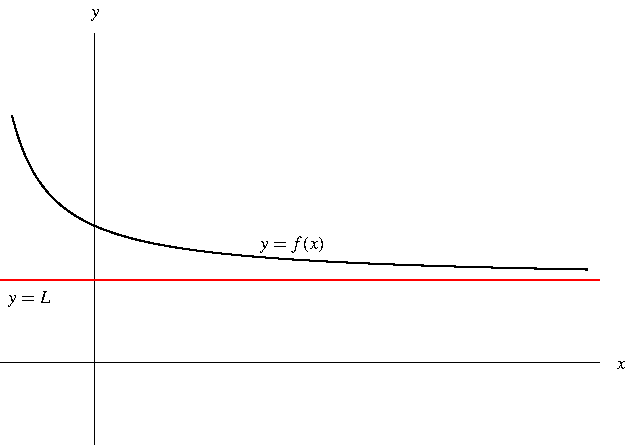
\includegraphics[width=4cm]{curve-sketching/pictures/04-04-asymptotesa.pdf}%
\column{.3\textwidth}
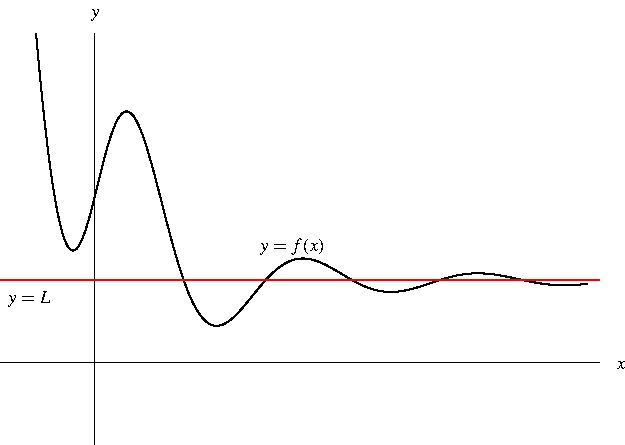
\includegraphics[width=4cm]{curve-sketching/pictures/04-04-asymptotesb.pdf}%
\column{.3\textwidth}
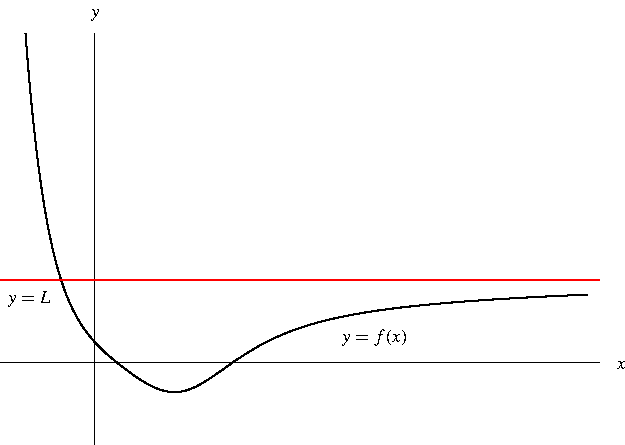
\includegraphics[width=4cm]{curve-sketching/pictures/04-04-asymptotesc.pdf}%
\end{columns}
}%
\begin{itemize}
\item<2->  There are many ways that this can happen.
\item<3->  Other notation: $f(x)\to L$ as $x\to \infty$.
\item<4->  $\infty$ is not a number.
\end{itemize}
\end{frame}



\begin{frame}[t]
\begin{definition}[Limit at Minus Infinity]
Let $f$ be a function defined on some interval $(- \infty , b)$.  Then
\[
\lim_{x\rightarrow -\infty} f(x) = L
\]
means that the values of $f$ can be made arbitrarily close to $L$ by taking $x$ sufficiently large negative.
\end{definition}
\begin{columns}[c]
\column{.5\textwidth}
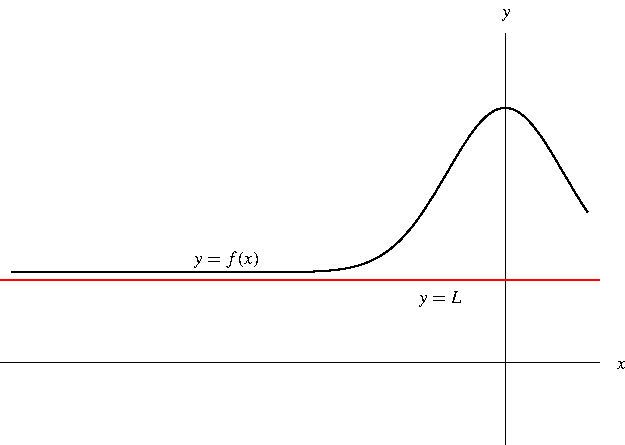
\includegraphics[width=6cm]{curve-sketching/pictures/04-04-negasymptotesa.pdf}%
\column{.5\textwidth}
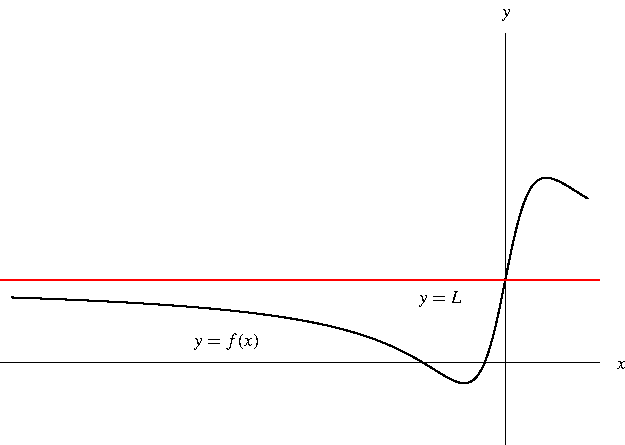
\includegraphics[width=6cm]{curve-sketching/pictures/04-04-negasymptotesb.pdf}%
\end{columns}
\end{frame}
% end module limit-at-infinity-def
